\documentclass[zh]{nccuthesis}

\usepackage{times}
\usepackage{verbatim}
\usepackage{color}
\usepackage{url}
\usepackage{graphicx}
\usepackage{array}
\usepackage{pdfpages} % include outside .pdf
\usepackage{wallpaper} % watermark
% for table generate
\usepackage{mathtools}
\usepackage{amsmath}
\usepackage{amssymb}
\usepackage{booktabs}
\usepackage{adjustbox}

\usepackage{multirow}
\usepackage{multicol}

% https://www.overleaf.com/learn/latex/How_to_Write_a_Thesis_in_LaTeX_(Part_3)%3A_Figures%2C_Subfigures_and_Tables
\usepackage{caption}
\usepackage{subcaption}

% Format the refs
%\usepackage[sort,comma]{natbib}
\usepackage[square,sort,comma,numbers]{natbib} % for ieee format [] , wei
\usepackage[hidelinks]{hyperref}

% For the tree
\usepackage{tikz}
\usepackage{tikz-qtree}

% For barchart
\usepackage{pgfplots}
\usepackage{notoccite}% PREVENTS CITES IN CAPTIONS FROM MISNUMBERING YOUR REFERENCES, wei

\usepackage{tabularx}

% Using the tex-text mapping for ligatures etc.
\defaultfontfeatures{Mapping=tex-text}

% Set the default fonts
\setmainfont{Times New Roman}
\setCJKmainfont{TW-Kai}

% Your information goes here
% author: Ray Lu
% ----------------------------------------------------------------------------
% "THE CHOCOLATE-WARE LICENSE":
% Tz-Huan Huang originally wrote this file. As long as you retain this notice you
% can do whatever you want with this stuff. If we meet some day, and you think
% this stuff is worth it, you can buy me a chocolate in return Tz-Huan Huang
% ----------------------------------------------------------------------------


% 若需在封面加入英文資訊,可在下方第一個{}中進行修改,若是需要顯示學院名稱,僅須將%\college前的‘%’去除後再重新編譯即可。
%下方{}內資訊及為封面資訊設定,可自由進行修改,若需顯示英文資訊可至nccuthesisi.cls中查看相關說明。

% Syntax: \var{English}{Chinese}
\university{National Chengchi University}{國立政治大學}
%\college{College of Social Science}{社會科學院}
\institute{Department of Computer Science}{資訊科學系}
\title{Thesis Topic Thesis Topic Thesis Topic Thesis Topic}{論文題目論文題目論文題目論文題目}
\author{}{OOO\ 撰}
\studentid{}
\advisor{}{OOO\ 博士 \\}
\defenseyear{2023}{一百一十二\ }
\defensemonth{June\ }{六\ }
\defenseday{}

\pgfplotsset{compat=1.14}
\begin{document}

% 政大論文浮水印
\input{src/without-watermark.tex}

\hypersetup{pageanchor=false}

\frontmatter
\pagenumbering{gobble}
\makecover

\clearpages
\setcounter{page}{1}
\hypersetup{pageanchor=true}
\pagenumbering{roman}
\phantomsection

% generate certification
% \makecertification
% or include scanned pdf


%\begin{acknowledgementszh}
謝謝謝謝。謝謝謝謝。謝謝謝謝。謝謝謝謝。謝謝謝謝。謝謝謝謝。謝謝謝謝。謝謝謝謝。謝謝謝謝。謝謝謝謝。謝謝謝謝。謝謝謝謝。謝謝謝謝。謝謝謝謝。謝謝謝謝。謝謝謝謝。謝謝謝謝。謝謝謝謝。謝謝謝謝。謝謝謝謝。謝謝謝謝。謝謝謝謝。謝謝謝謝。謝謝謝謝。謝謝謝謝。謝謝謝謝。謝謝謝謝。謝謝謝謝。謝謝謝謝。謝謝謝謝。謝謝謝謝。謝謝謝謝。謝謝謝謝。謝謝謝謝。謝謝謝謝。謝謝謝謝。謝謝謝謝。謝謝謝謝。謝謝謝謝。謝謝謝謝。謝謝謝謝。謝謝謝謝。謝謝謝謝。謝謝謝謝。謝謝謝謝。謝謝謝謝。謝謝謝謝。謝謝謝謝。謝謝謝謝。謝謝謝謝。謝謝謝謝。謝謝謝謝。謝謝謝謝。謝謝謝謝。謝謝謝謝。謝謝謝謝。謝謝謝謝。謝謝謝謝。謝謝謝謝。謝謝謝謝。謝謝謝謝。謝謝謝謝。謝謝謝謝。謝謝謝謝。謝謝謝謝。謝謝謝謝。謝謝謝謝。謝謝謝謝。謝謝謝謝。謝謝謝謝。謝謝謝謝。謝謝謝謝。謝謝謝謝。謝謝謝謝。謝謝謝謝。謝謝謝謝。謝謝謝謝。謝謝謝謝。謝謝謝謝。謝謝謝謝。謝謝謝謝。謝謝謝謝。謝謝謝謝。謝謝謝謝。謝謝謝謝。謝謝謝謝。謝謝謝謝。謝謝謝謝。謝謝謝謝。謝謝謝謝。謝謝謝謝。謝謝謝謝。謝謝謝謝。謝謝謝謝。謝謝謝謝。謝謝謝謝。謝謝謝謝。\par


\begin{flushright}
OOO  \qquad 謹致於\par

國立政治大學資訊科學研究所\par

中華民國一一二年六月\par

\end{flushright}

\end{acknowledgementszh}



%%中英文摘要皆寫於本檔案即可abstractzh下方撰寫中文摘要 abstracten下方撰寫英文摘要。

\begin{abstractzh}

摘要摘要。摘要摘要。摘要摘要。摘要摘要。摘要摘要。摘要摘要。摘要摘要。摘要摘要。摘要摘要。摘要摘要。摘要摘要。摘要摘要。摘要摘要。摘要摘要。摘要摘要。摘要摘要。摘要摘要。摘要摘要。摘要摘要。摘要摘要。摘要摘要。摘要摘要。摘要摘要。摘要摘要。摘要摘要。摘要摘要。摘要摘要。摘要摘要。摘要摘要。摘要摘要。摘要摘要。摘要摘要。摘要摘要。摘要摘要。摘要摘要。摘要摘要。摘要摘要。摘要摘要。摘要摘要。摘要摘要。摘要摘要。摘要摘要。摘要摘要。摘要摘要。摘要摘要。摘要摘要。摘要摘要。摘要摘要。摘要摘要。摘要摘要。摘要摘要。摘要摘要。摘要摘要。摘要摘要。摘要摘要。摘要摘要。摘要摘要。摘要摘要。摘要摘要。摘要摘要。摘要摘要。摘要摘要。摘要摘要。摘要摘要。摘要摘要。摘要摘要。摘要摘要。摘要摘要。摘要摘要。摘要摘要。摘要摘要。摘要摘要。摘要摘要。摘要摘要。摘要摘要。摘要摘要。摘要摘要。摘要摘要。摘要摘要。摘要摘要。摘要摘要。摘要摘要。摘要摘要。摘要摘要。摘要摘要。摘要摘要。摘要摘要。摘要摘要。摘要摘要。摘要摘要。摘要摘要。摘要摘要。摘要摘要。摘要摘要。摘要摘要。摘要摘要。摘要摘要。摘要摘要。摘要摘要。摘要摘要。摘要摘要。摘要摘要。摘要摘要。摘要摘要。摘要摘要。摘要摘要。摘要摘要。摘要摘要。摘要摘要。摘要摘要。摘要摘要。

~\\
\noindent
關鍵字:關鍵字、關鍵字、關鍵字、關鍵字
\end{abstractzh}

\begin{abstracten}
\begin{small}
Abstract abstract. Abstract abstract. Abstract abstract. Abstract abstract. Abstract abstract. Abstract abstract. Abstract abstract. Abstract abstract. Abstract abstract. Abstract abstract. Abstract abstract. Abstract abstract. Abstract abstract. Abstract abstract. Abstract abstract. Abstract abstract. Abstract abstract. Abstract abstract. Abstract abstract. Abstract abstract. Abstract abstract. Abstract abstract. Abstract abstract. Abstract abstract. Abstract abstract. Abstract abstract. Abstract abstract. Abstract abstract. Abstract abstract. Abstract abstract. Abstract abstract. Abstract abstract. Abstract abstract. Abstract abstract. Abstract abstract. Abstract abstract. Abstract abstract. Abstract abstract. Abstract abstract. Abstract abstract. Abstract abstract. Abstract abstract. Abstract abstract. Abstract abstract. Abstract abstract. Abstract abstract. Abstract abstract. Abstract abstract. Abstract abstract. Abstract abstract. Abstract abstract. Abstract abstract. Abstract abstract. Abstract abstract. Abstract abstract. Abstract abstract. Abstract abstract. Abstract abstract. Abstract abstract. Abstract abstract. Abstract abstract. Abstract abstract. Abstract abstract. Abstract abstract. Abstract abstract. Abstract abstract.


~\\
\noindent
Keywords: Keyword, Keyword, Keyword, Keyword
\end{small}
\end{abstracten}


\newenvironment{changemargin}[2]{%
\begin{list}{}{

\setlength{\topmargin}{#1}
\setlength{\footskip}{#2}
}%
\item[]}{\end{list}}
% Table of Content
\clearpages
\begin{changemargin}{-2cm}{2.5cm}
\begin{small}
\tableofcontents
\end{small}
\end{changemargin}

% List of Figures
% add by WEI 讓目錄增加前綴圖
\newcommand{\loflabel}{圖}
\renewcommand{\numberline}[1]{\loflabel~#1\hspace*{1em}}

\clearpages
\listoffigures
% List of Tables

\newcommand{\lotlabel}{表}
\renewcommand{\numberline}[1]{\lotlabel~#1\hspace*{1em}}

\clearpages
\listoftables

\mainmatter

%%有需要增加或減少章節就記得來這邊更改

% Your thesis goes here
\chapter{緒論}  %可更改{}中的文字來更改大標題名稱
\label{c:intro}

%若想新增新的節可用\section{}來加入
%段落結束後可使用\par來結束段落

\section{研究背景}

研究背景研究背景研究背景研究背景研究背景。研究背景研究背景研究背景研究背景研究背景。研究背景研究背景研究背景研究背景研究背景。研究背景研究背景研究背景研究背景研究背景。研究背景研究背景研究背景研究背景研究背景。研究背景研究背景研究背景研究背景研究背景。研究背景研究背景研究背景研究背景研究背景。研究背景研究背景研究背景研究背景研究背景\cite{01}。研究背景研究背景研究背景研究背景研究背景。研究背景研究背景研究背景研究背景研究背景。研究背景研究背景研究背景研究背景研究背景\cite{02, 14}。

\section{研究動機與目的}

圖\ref{i:uav_method}動機動機動機動機動機動機動機動機動機動機動機動機動機動機動機動機動機,動機動機動機動機動機動機動機,圖\ref{i:uav_method1}動機動機動機動機動機動機動機,圖\ref{i:uav_method2}動機動機動機動機動機動機動機動機。

\section{研究成果與貢獻}
成果貢獻成果貢獻成果貢獻成果貢獻成果貢獻成果貢獻成果貢獻成果貢獻成果貢獻成果貢獻成果貢獻成果貢獻成果貢獻成果貢獻成果貢獻成果貢獻成果貢獻成果貢獻成果貢獻成果貢獻成果貢獻成果貢獻成果貢獻成果貢獻成果貢獻成果貢獻成果貢獻成果貢獻成果貢獻成果貢獻成果貢獻成果貢獻成果貢獻成果貢獻。

\section{論文架構}
架構架構架構架構架構架構架構架構架構架構架構架構架構架構架構架構架構架構架構架構架構架構架構架構架構架構架構架構架構架構架構架構架構架構架構架構架構架構架構架構架構架構。

\chapter{文獻探討}
文獻探討文獻探討文獻探討文獻探討文獻探討文獻探討文獻探討文獻探討文獻探討文獻探討文獻探討文獻探討文獻探討文獻探討文獻探討文獻探討文獻探討文獻探討文獻探討文獻探討文獻探討。

\section{文獻文獻}

\subsection{探討探討}

PID控制器為被廣泛應用的控制器,公式\label{f:pid}為其數學公式。公式公式公式公式公式公式公式公式公式公式公式公式公式公式公式公式公式公式公式公式公式公式公式公式公式公式公式公式公式公式公式公式公式公式公式公式公式公式。

\begin{equation}
u(t) = K_P e(t) + K_I\int_{0}^{t} e(\tau) d\tau + K_D\frac{de(t)}{dt} \label{f:pid}
\end{equation}














































\chapter{技術方法}

方法方法方法方法方法方法方法方法方法方法方法方法方法方法方法方法方法方法方法方法方法方法方法方法方法方法方法方法方法方法方法方法方法方法方法方法方法方法方法方法方法方法方法方法方法方法方法方法方法方法方法方法方法方法方法方法方法方法。

\section{系統架構}
模組模組模組模組模組模組模組模組模組模組模組模組模組模組。模組模組模組模組模組模組模組模組模組模組模組模組模組模組。模組模組模組模組模組模組模組模組模組模組模組模組模組模組。模組模組模組模組模組模組模組模組模組模組模組模組模組模組。

\subsection{方程式測試}
如公式\ref{f:1}所示,公式公式公式公式公式公式公式公式公式公式公式公式公式公式公式,公式公式公式公式公式公式公式公式公式公式。

\begin{equation}
\begin{aligned}
x_{pos} = \sum_{i=1}^{T} x_{v_{i}} \cdot \Delta t \\
y_{pos} = \sum_{i=1}^{T} y_{v_{i}}  \cdot \Delta t \label{f:1}
\end{aligned}
\end{equation}


\chapter{實驗結果與分析}
\label{c:implement}

\section{實驗設置}

\subsection{表格表格}
表\ref{4-1}為相關規格。設置設置設置設置設置設置設置設置設置設置設置設置設置設置設置設置設置設置設置設置設置設置設置設置設置設置設置設置設置設置設置設置設置設置設置設置設置設置。

\begin{table}[htbp]

\caption{表格表格表格}
\begin{center}
\tiny
%務必在下方{}中加上表格章節編號
\label{4-1}
\begin{adjustbox}{width=0.8\textwidth}
\begin{tabular}[c]{|c|c|c|}
    \hline
    參數 & ANAFI 4K & ANAFI Thermal \\
    \hline
    尺寸 & 242x315x65 mm & 242x315x64 mm \\
    \hline
    重量 &  320 g & 315 g \\
    \hline
     續航時間 & 25 min & 26 min \\
     \hline
     串流影像解析度  & \multicolumn{2}{c|}{1280x720 px (720 p)} \\
    \hline
\end{tabular}
\end{adjustbox}
\end{center}

\end{table}

\section{真實環境實驗}
實驗實驗實驗實驗實驗實驗實驗實驗實驗實驗實驗實驗實驗實驗實驗實驗實驗實驗實驗實驗實驗實驗實驗實驗實驗實驗實驗實驗實驗實驗實驗實驗實驗實驗實驗實驗實驗實驗實驗實驗實驗實驗實驗實驗實驗實驗實驗實驗實驗實驗實驗實驗實驗實驗實驗實驗實驗實驗實驗實驗實驗實驗。

\subsection{實驗結果分析}
結果結果結果結果結果結果結果結果結果結果結果結果結果結果結果結果結果結果結果結果結果結果結果結果結果結果結果結果結果結果結果結果結果結果結果結果結果結果結果結果結果結果結果結果結果結果結果結果結果結果結果結果結果結果結果。

\begin{itemize}
\item
\textbf{分析分析}
\end{itemize}

分析分析分析分析分析分析分析分析分析分析分析分析分析分析分析分析分析分析分析分析分析分析分析分析分析分析分析分析分析分析分析分析分析分析分析分析分析分析分析分析分析分析分析分析分析分析分析分析分析分析分析分析分析分析分析分析分析分析分析分析分析分析分析分析分析分析分析分析分析分析分析分析分析分析分析分析分析分析分析分析分析分析分析分析分析分析分析分析分析分析分析分析分析分析分析分析分析分析分析分析分析分析分析分析分析分析分析分析分析分析。

\newpage
\begin{figure}[!htbp]
  \centering
  \begin{subfigure}{1.0\textwidth}
    \centering
    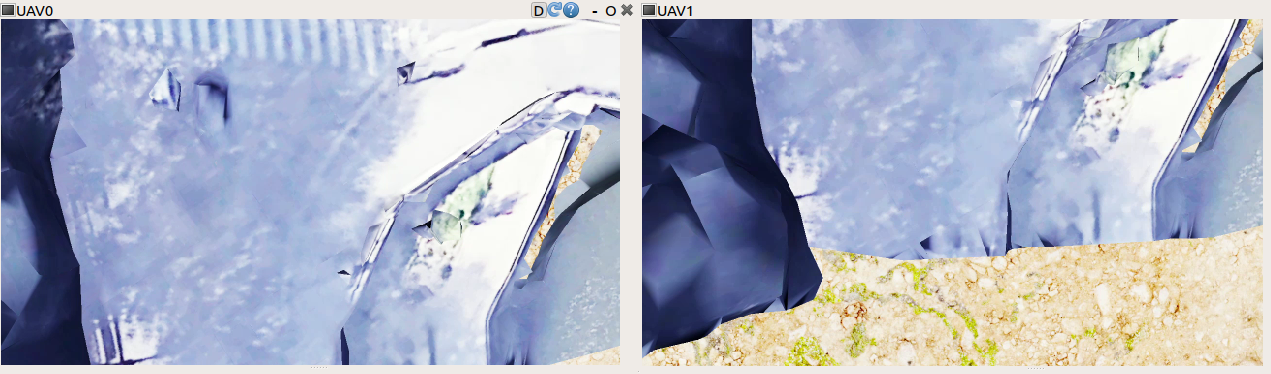
\includegraphics[width=\linewidth]{images/sim25_2.png}
    \caption{子圖A}
  \end{subfigure}
  \vspace{1em}
  
  \begin{subfigure}{1.0\textwidth}
    \centering
    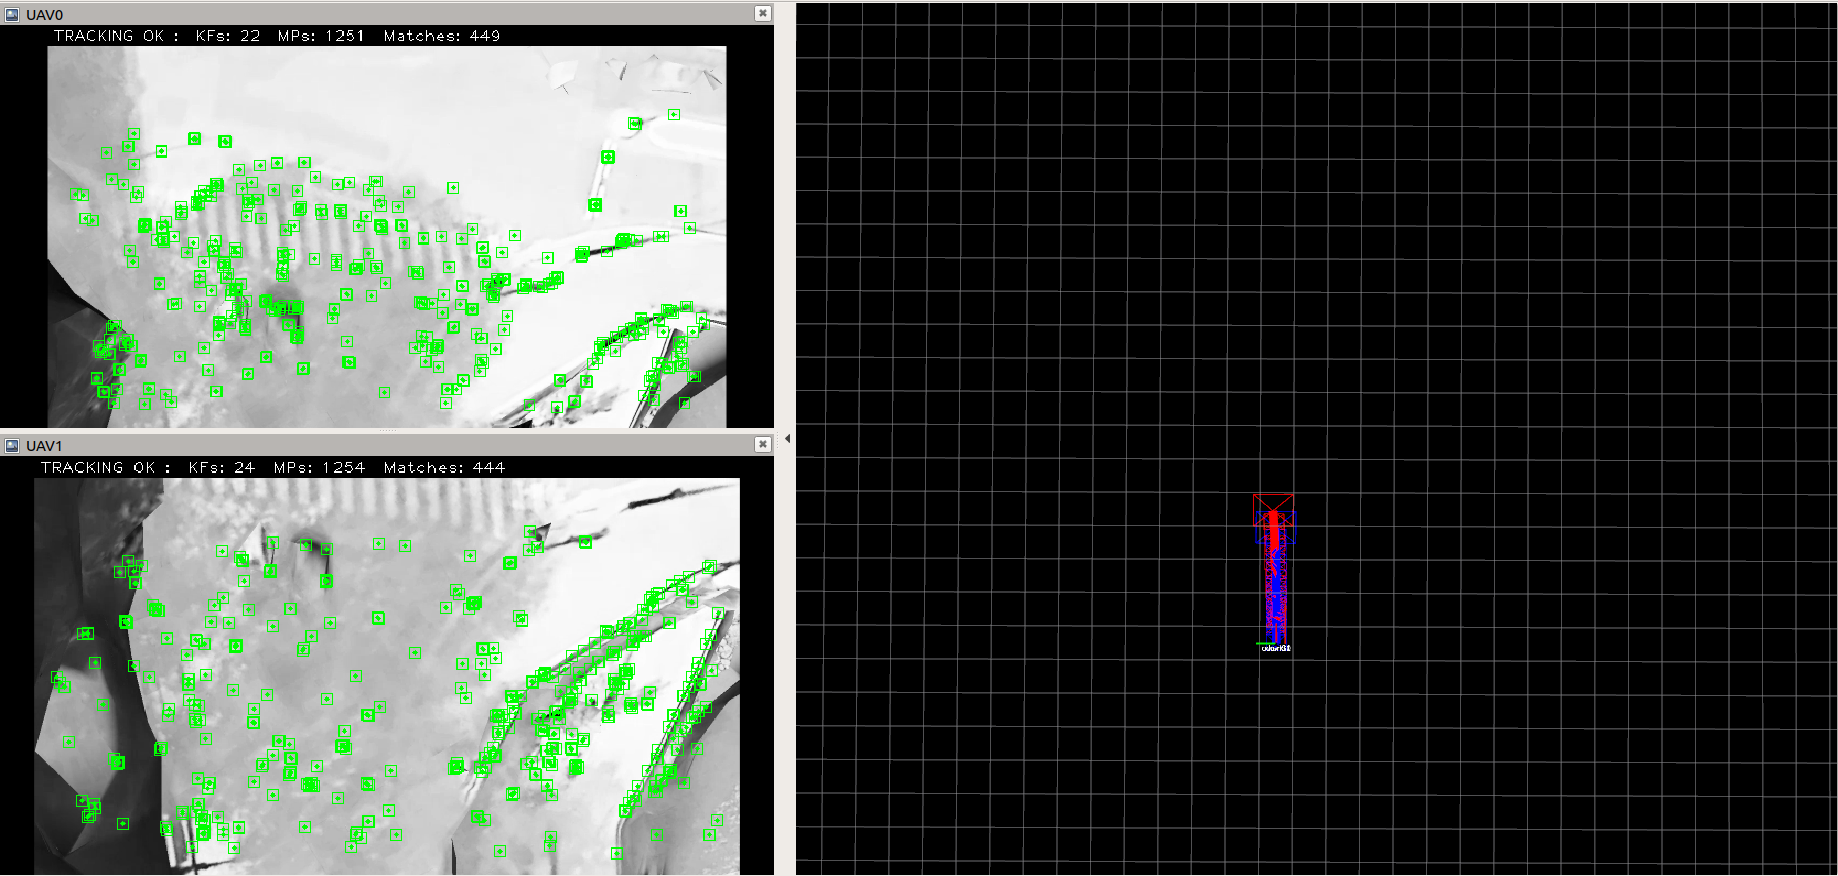
\includegraphics[width=\linewidth]{images/sim25_3.png}
    \caption{子圖B}
  \end{subfigure}
  \vspace{1em}
  
  \begin{subfigure}{1.0\textwidth}
    \centering
    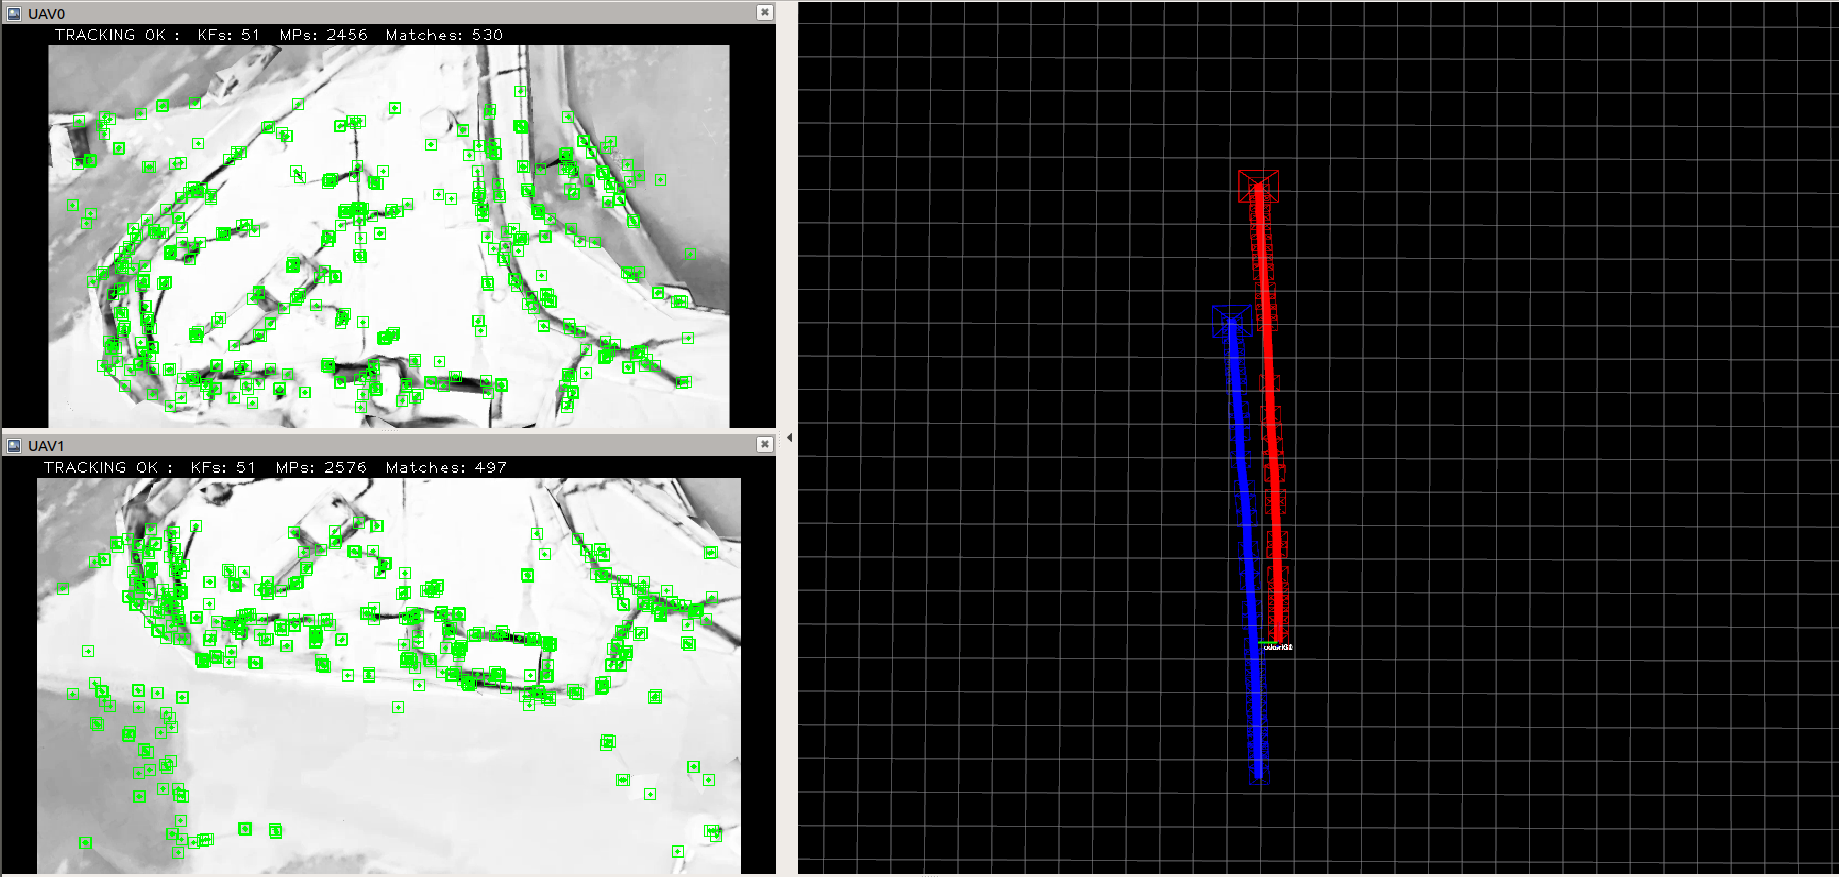
\includegraphics[width=\linewidth]{images/sim25_4.png}
    \caption{子圖C}
  \end{subfigure}
  \caption{圖片圖片圖片}
  \label{i:sim25_slam}
\end{figure}

\newpage

分析分析分析分析分析分析分析分析分析分析分析分析分析分析分析分析分析分析分析分析分析分析分析分析分析分析分析分析分析分析分析分析分析分析分析分析分析分析分析分析分析分析分析分析分析分析分析分析分析分析分析分析分析分析分析分析分析分析分析分析分析分析分析分析分析分析分析分析分析分析分析分析分析分析分析分析分析分析分析分析分析分析分析分析分析分析分析分析分析分析分析分析分析分析分析分析分析分析分析分析分析分析分析分析分析分析分析分析分析分析分析分析分析分析分析分析分析分析分析分析分析分析分析分析分析分析分析分析分析分析分析分析分析分析。

\begin{table}[H]
\centering
\caption{結果結果結果結果結果結果結果結果}
\label{t:sim30_5times}
\begin{tabularx}{\textwidth}{|c|X|X|c|}
\hline
\multirow{2}{*}{} & \multicolumn{2}{c|}{平均橫向誤差 (m)} & \multirow{2}{*}{平均縱向誤差 (m)} \\ \cline{2-3}
 & \multicolumn{1}{X|}{\centering UAV0} & \multicolumn{1}{X|}{\centering UAV1} &  \\ \hline
實驗1 & \multicolumn{1}{c|}{0.001} &  \multicolumn{1}{c|}{0.001} & 0.001 \\ \hline
實驗2 & \multicolumn{1}{c|}{0.001} &  \multicolumn{1}{c|}{0.001} & 0.001 \\ \hline
實驗3 & \multicolumn{1}{c|}{0.001} &  \multicolumn{1}{c|}{0.001} & 0.001 \\ \hline
實驗4 & \multicolumn{1}{c|}{0.001} &  \multicolumn{1}{c|}{0.001} & 0.001 \\ \hline
實驗5 & \multicolumn{1}{c|}{0.001} &  \multicolumn{1}{c|}{0.001} & 0.001 \\ \hline
\end{tabularx}
\end{table}

\begin{table}[H]
\centering
\caption{表格表格表格表格表格表格}
\label{t:sim30_with_no_formation}
\begin{tabularx}{\textwidth}{|c|X|X|c|}
\hline
\multirow{2}{*}{} & \multicolumn{2}{c|}{平均橫向誤差 (m)} & \multirow{2}{*}{平均縱向誤差 (m)} \\ \cline{2-3}
 & \multicolumn{1}{X|}{\centering UAV0} & \multicolumn{1}{X|}{\centering UAV1} &  \\ \hline
無應用策略 & \multicolumn{1}{c|}{0.002} &  \multicolumn{1}{c|}{0.002} & 0.002 \\ \hline
有應用策略 & \multicolumn{1}{c|}{0.001} &  \multicolumn{1}{c|}{0.001} &  \textbf{0.001} \\ \hline
\end{tabularx}
\end{table}

\newpage

\section{小結}
小結小結小結小結小結小結小結小結小結小結小結小結小結小結小結小結小結小結小結小結小結小結小結小結小結小結小結小結小結小結小結小結小結小結小結小結小結小結小結小結小結小結小結小結小結小結小結小結小結小結小結小結小結小結小結小結小結小結小結小結小結小結小結小結小結小結小結小結小結小結小結小結小結小結小結小結小結小結小結小結小結小結小結小結小結小結小結小結小結。
\chapter{結論與未來展望}
\label{c:experiment}
結論結論結論。結論結論結論。結論結論結論。結論結論結論。結論結論結論。結論結論結論。結論結論結論。結論結論結論。結論結論結論。結論結論結論。結論結論結論。結論結論結論。結論結論結論。結論結論結論。結論結論結論。結論結論結論。結論結論結論。結論結論結論。

\section{研究結論}

研究結論,研究結論,研究結論,研究結論,研究結論,研究結論,研究結論,研究結論,研究結論,研究結論,研究結論,研究結論,研究結論:

\begin{itemize}
\item[1.] 研究結論。研究結論。研究結論。研究結論。研究結論。研究結論。
\end{itemize}

\begin{itemize}
\item[2.] 研究結論。研究結論。研究結論。研究結論。研究結論。研究結論。
\end{itemize}

\begin{itemize}
\item[3.] 研究結論。研究結論。研究結論。研究結論。研究結論。研究結論。
\end{itemize}

\section{未來展望}
研究結論,研究結論,研究結論,研究結論,研究結論,研究結論,研究結論,研究結論,研究結論,研究結論,研究結論,研究結論,研究結論:

\begin{itemize}
\item[1.] 未來展望。未來展望。未來展望。未來展望。未來展望。未來展望。
\end{itemize}

\begin{itemize}
\item[2.]  未來展望。未來展望。未來展望。未來展望。未來展望。未來展望。
\end{itemize}

\begin{itemize}
\item[3.] 未來展望。未來展望。未來展望。未來展望。未來展望。未來展望。
\end{itemize}


\@startappendix


\backmatter

\clearpages
\phantomsection
\addcontentsline{toc}{chapter}{\bibname}
\bibliographystyle{ieeetr} % IEEE format
% Your bibliography goes here
\bibliography{thesis}

\end{document}
